\documentclass[11pt,a4paper]{article}
% \usepackage[backed=bibtex]{biblatex}
\usepackage[hyperref]{acl2021}
\usepackage{times}
\usepackage{latexsym}
\usepackage{amssymb,amsmath}
\usepackage{graphicx}
\usepackage{microtype}
\usepackage{csvsimple}
\usepackage{booktabs}
\usepackage{siunitx}
\usepackage{hyperref}
\usepackage{array}
\usepackage{tabularx}
\usepackage{subcaption}


\usepackage{tabulary}

% \renewcommand{\UrlFont}{\ttfamily\small}
\usepackage[margin=2cm]{geometry}
% This is not strictly necessary, and may be commented out,
% but it will improve the layout of the manuscript,
% and will typically save some space.
% \usepackage[backend=bibtex]{microtype}
%\aclfinalcopy % Uncomment this line for the final submission
%\def\aclpaperid{***} %  Enter the acl Paper ID her
%\setlength\titlebox{5cm}

% \newcommand\BibTeX{B\textsc{ib}\TeX}

\aclfinalcopy


% \renewcommand{\UrlFont}{\ttfamily\small}
% \aclfinalcopy % Uncomment this line for the final submission
%\def\aclpaperid{***} %  Enter the acl Paper ID here
%\setlength\titlebox{5cm}

\title{NIR Project}


\author{Nicklas Sambleben \\
  \texttt{WKL296} \\ }

\date{}

\begin{document}
\maketitle

\section{Dateset and Indexing}

\subsection*{Dataset}
We obtained the following statistics

\begin{table}[htbp]
    \centering
    \label{tab:statistics}
    \begin{tabular}{lcc}
        \toprule
        \multicolumn{1}{c}{\textbf{Statistic}} & \multicolumn{1}{c}{\textbf{Documents}} & \multicolumn{1}{c}{\textbf{Queries}} \\
        \midrule
        Total                                  & 3,213,835                              & 367,013                              \\
        Min                                    & 0                                      & 1                                    \\
        Max                                    & 2,064,096                              & 38                                   \\
        Median                                 & 3,577                                  & 6                                    \\
        Average                                & 6,996.61                               & 5.95                                 \\
        \bottomrule
    \end{tabular}
    \caption{Document and Query Statistics}
\end{table}

The statistics provided shed illuminating light on the key
characteristics of the MS MARCO dataset, which is composed of over
3.2 million documents and 367,013 queries. This large-scale dataset
offers a substantial and diverse corpus for developing and testing
information retrieval systems. However, certain aspects of the data
distribution warrant further scrutiny and careful consideration
during the modeling process.

Regarding the document corpus, we observe that the document length
varies dramatically, ranging from 0 to over 2 million words. The
presence of documents with a length of zero is particularly
intriguing, possibly indicating the existence of empty or corrupted
entries within the dataset. Such instances could inadvertently impact
the performance and interpretability of the models and, as such, it
is advisable to inspect these documents further and decide on a
suitable strategy for their inclusion or removal.

Moreover, the upper end of the document length distribution also
reveals outliers, with the maximum length exceeding 2 million words.
Documents of such extraordinary length may not represent typical
instances and could potentially skew model performance or learning.
Therefore, it would be prudent to investigate the nature of these
long documents to ensure they don't contain repetitive or irrelevant
information, and to assess their impact on the modeling process.

The median and average document lengths, at approximately 3577 and
7000 words respectively, suggest a diverse document length
distribution. This variation is likely to expose models to a wide
range of document structures and contents, thereby contributing to
their robustness.

Turning our attention to the queries, the dataset presents a broad
spectrum of search intents as reflected by the query lengths ranging
from 1 to 38 words. The brevity of the shortest queries underscores
the inherent challenge in information retrieval: discerning user
intent from minimal input. On the other hand, the longest queries are
surprisingly detailed, indicating more complex or specific user
information needs.

The average and median lengths of queries hover around 6 words,
aligning with expectations for search query distributions and
underscoring the need for models capable of understanding and
retrieving relevant information for a wide range of query
complexities.

In conclusion, the MS MARCO dataset presents a rich and varied
resource for developing and refining information retrieval systems.
However, certain peculiarities in the data distribution, such as
potentially empty documents and extremely long documents, necessitate
careful preprocessing and scrutiny. Similarly, the diversity in query
length calls for models that can adeptly handle a broad spectrum of
user intents. With meticulous data handling and appropriate modeling
strategies, this dataset offers fertile ground for advancements in
the field of information retrieval.
\begin{figure}[ht!]
    \centering
    \begin{subfigure}[b]{0.45\textwidth}
        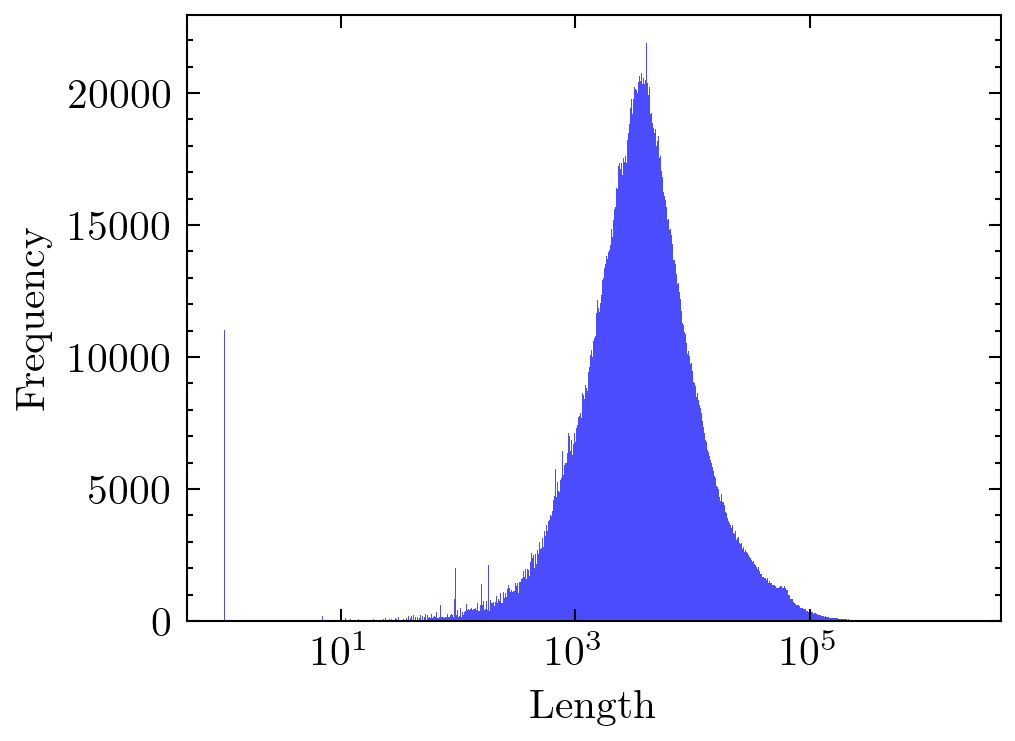
\includegraphics[width=\textwidth]{../media/doc_lengths_histogram_log_x.png}
        \caption{Histogram of document lengths (log x-axis)}
    \end{subfigure}
    \hfill
    \begin{subfigure}[b]{0.45\textwidth}
        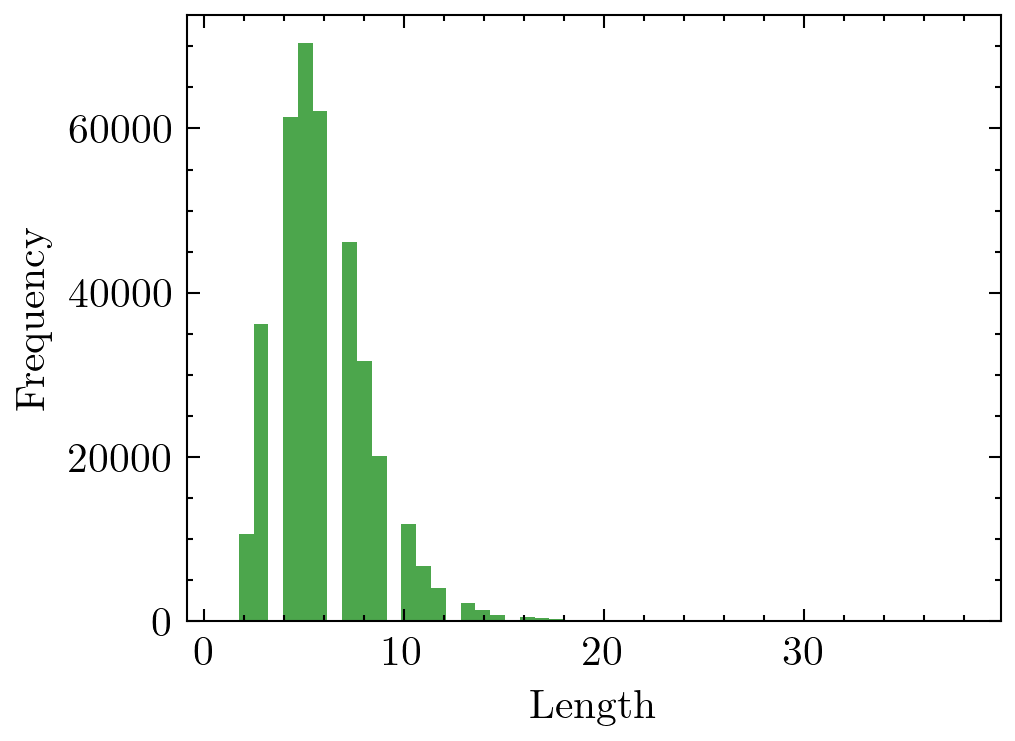
\includegraphics[width=\textwidth]{../media/query_lengths_histogram.png}
        \caption{Histogram of query lengths}
    \end{subfigure}
    \caption{Histograms of document and query lengths}
\end{figure}

\begin{figure}[ht!]
    \centering
    \begin{subfigure}[b]{0.45\textwidth}
        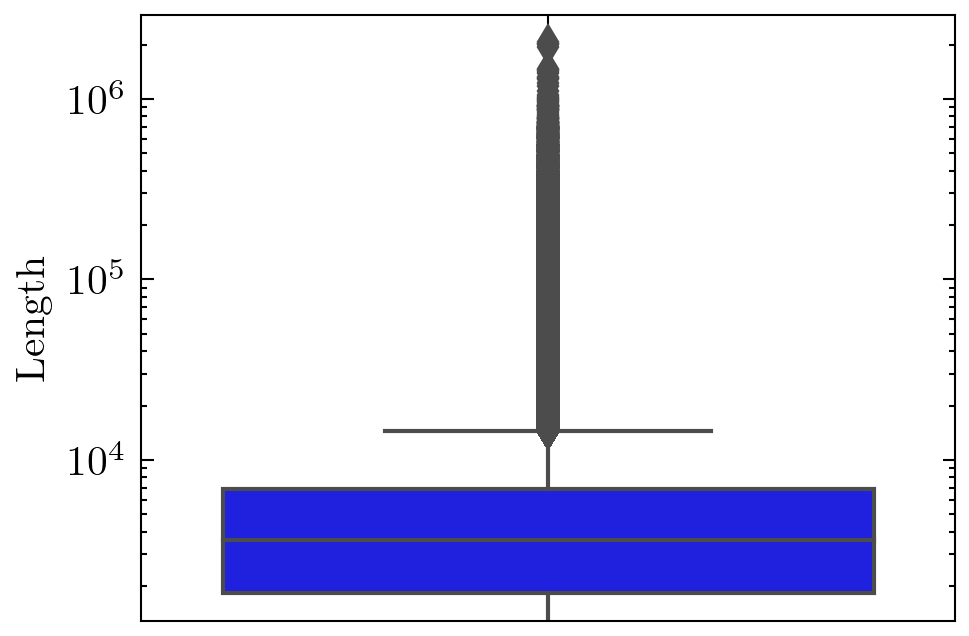
\includegraphics[width=\textwidth]{../media/doc_lengths_boxplot_log_y.png}
        \caption{Box plot of document lengths (log y-axis)}
    \end{subfigure} 
    \hfill
    \begin{subfigure}[b]{0.45\textwidth}
        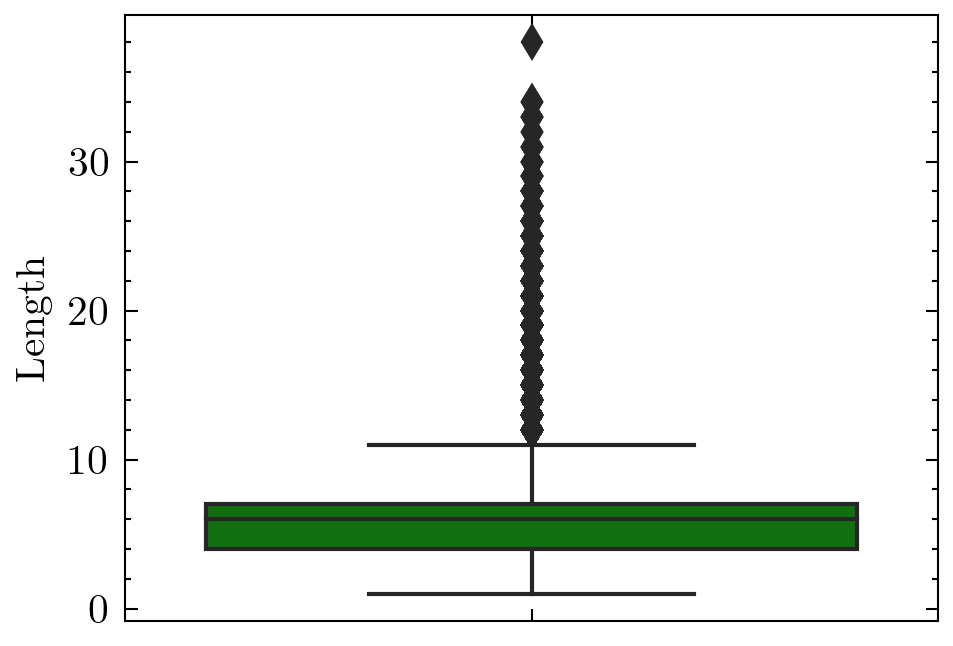
\includegraphics[width=\textwidth]{../media/query_lengths_boxplot.png}
        \caption{Box plot of query lengths}
    \end{subfigure}
    \caption{Boxplots of document and query lengths}
\end{figure}

\newpage

\subsection{Indexing}
When discussing the results of our indexing strategies for the
MSMARCO dataset, several points come to light. Four different types
of indexes were created: a full index, one with stopwords removed,
one employing stemming, and a combination of stopwords removed and
stemming.

\begin{table}[htbp]
    \centering
    \caption{Document and Query Statistics}
    \label{tab:statistics}
    \begin{tabular}{lcc}
        \toprule
        \multicolumn{1}{c}{\textbf{Statistic}} & \multicolumn{1}{c}{\textbf{Documents}} & \multicolumn{1}{c}{\textbf{Queries}} \\
        \midrule
        Total                                  & 3,213,835                              & 367,013                              \\
        Min                                    & 0                                      & 1                                    \\
        Max                                    & 2,064,096                              & 38                                   \\
        Median                                 & 3,577                                  & 6                                    \\
        Average                                & 6,996.61                               & 5.95                                 \\
        \bottomrule
    \end{tabular}
\end{table}

We obtained the statistics for each index as shown in table
\ref{tab:mytable}.

The time taken to build each index varied. As expected, the full
index, which did not undergo any form of preprocessing, was the
quickest to construct. This is because both the removal of stopwords
and the application of stemming introduce additional computational
complexity. Nevertheless, the added time taken for these processes
can be justified when considering the potential benefits such as
reduced index size and potentially improved retrieval performance.

All index variants processed the same number of documents, which was
to be expected as the entire corpus was to be processed in each case.

The total number of terms displayed a significant reduction when
stopwords were removed. This can be attributed to the omission of
frequently occurring words, which generally do not contribute to the
semantic relevance of a document. On the other hand, the total number
of terms remained constant when only stemming was applied. This
demonstrates that stemming does not inherently reduce the number of
unique terms in an index, but standardizes them instead.

In terms of index size, the smallest was observed when both stopwords
were removed and stemming was applied. This indicates the potential
of these techniques to compress the size of an index. A smaller index
size can lead to faster query processing times and less memory usage,
which can be significant advantages for large-scale information
retrieval systems.

However, the average search time was not the smallest for the
stopwords removed stemming variant. This suggests that the additional
computational costs of processing stemmed terms and handling
stopwords during query processing may offset the advantages of a
reduced index size in terms of search speed. In fact, the full index
variant, despite having the largest index size, returned the fastest
average search times.

In conclusion, the choice of an indexing strategy heavily depends on
the specific requirements of the information retrieval system. If
memory capacity is a concern, then an indexing strategy that employs
stopword removal and stemming might be a better choice due to the
significant reduction in index size. However, if the speed of search
is a primary concern, an indexing strategy without these
preprocessing steps might be more beneficial, given the computational
overhead these steps introduce during query processing. This analysis
does not consider retrieval effectiveness, which is another crucial
factor in choosing an indexing strategy. Further research would be
needed to explore the impact of these indexing strategies on
retrieval effectiveness.

\section{Ranking Models and Evaluation}

The evaluation and ranking of the four indexing models were carried
out using two different ranking models: Okapi BM25 and Language Model
(LM). We used Pyserini, a python interface to the Anserini IR
toolkit, for creating and evaluating these models. We chose this
library for its cutting-edge capabilities in information retrieval
tasks and its easy integration with Python.

For model tuning and evaluation, we employed a Group 5-Fold Cross
Validation approach. This technique ensures that the same query does
not appear in both the training and validation sets in each fold,
thereby preventing data leakage between these sets. This method is a
variant of the traditional k-fold cross-validation technique and is
particularly useful when data includes groups or clusters. In our
case, the group was formed by the unique queries.

The Group K-Fold Cross Validation technique partitions the data into
'k' equal-sized groups or 'folds'. We set aside each unique group as
a test set while using the remaining groups as a training set. We
then trained our model on the training set and evaluated it on the
reserved test set. This process was repeated 'k' times so that each
group was used as a test set exactly once. We then averaged the
results from each of the 'k' experiments to provide a more
comprehensive and robust measure of model performance.

The use of Group K-Fold Cross Validation, together with
hyperparameter tuning through grid search, allowed us to
systematically explore the performance of different model
configurations. This approach provided valuable insights into how the
choice of parameters and ranking models affects retrieval
performance. It not only helped us identify the optimal configuration
but also improved our understanding of how these models behave under
different settings.

We statistics for each of the four indexing and models can be seen in the table
\ref{tab:performance}.

\begin{table*}[htbp]
    \centering
    \begin{tabulary}{\textwidth}{L L L C C C C C C C C}
        \toprule
        \textbf{Index} & \textbf{Model} & \textbf{Best Config.} & \textbf{NDCG} & \textbf{MRR} & \textbf{P@5} & \textbf{P@10} & \textbf{P@20} & \textbf{Recall@5} & \textbf{Recall@10} & \textbf{Mean Resp. Time} \\
        \midrule
        full index & bm25 & k1: 0.9, b: 0.6 & 0.019 & 0.006 & 0.004 & 0.002 & 0.032 & 0.043 & 0.043  & 0.001 \\
        full index & lm & mu: 1000 & 0.019 & 0.006 & 0.004 & 0.002 & 0.030 & 0.041 & 0.041 & 0.005 \\
        stopwords removed & bm25 & k1: 0.9, b: 0.6 & 0.020 & 0.006 & 0.004 & 0.002 & 0.032 & 0.044 & 0.044  & 0.000 \\
        stopwords removed & lm & mu: 1000 & 0.020 & 0.006 & 0.004 & 0.002 & 0.031 & 0.045 & 0.045  & 0.003 \\
        stemming & bm25 & k1: 0.9, b: 0.6 & 0.043 & 0.014 & 0.009 & 0.004 & 0.069 & 0.088 & 0.088  & 0.001 \\
        stemming & lm & mu: 1000 & 0.042 & 0.013 & 0.009 & 0.004 & 0.067 & 0.086 & 0.086  & 0.005 \\
        stopwords removed stemming & bm25 & k1: 0.9, b: 0.6 & 0.037 & 0.012 & 0.008 & 0.004 & 0.060 & 0.080 & 0.080  & 0.001 \\
        stopwords removed stemming & lm & mu: 1000 & 0.040 & 0.013 & 0.008 & 0.004 & 0.065 & 0.085 & 0.085  & 0.003 \\
        \bottomrule
    \end{tabulary}
    \caption{Retrieval Model Performance}
    \label{tab:performance}
\end{table*}

Using \ref{tab:performance},we conducted a comprehensive analysis and concluded that the
combination of stemming and the BM25 model is the most effective for
our given dataset and task. The Group K-Fold cross-validation
technique provided a reliable and robust validation of this finding.

We tuned the parameters for both BM25 and LM using grid search, a
hyperparameter tuning technique that methodically builds and
evaluates a model for each combination of algorithm parameters
specified in a grid. For BM25, the tuned hyperparameters were k1 and
b. For LM, the tuned hyperparameter was mu.

We used Normalized Discounted Cumulative Gain (NDCG), Mean Reciprocal
Rank (MRR), Precision, and Recall at 5, 10, and 20 cutoffs as
evaluation measures. We used NDCG@10 for model tuning. Each of these
metrics is widely used in information retrieval and provides a
comprehensive analysis of the performance of the ranking models.
However, each of these measures has its own limitations. For
instance, NDCG and MRR are rank-sensitive measures, unlike Precision
and Recall. On the other hand, Precision and Recall do not take into
account the rank of the relevant documents. Therefore, the
combination of these evaluation metrics gives a more complete
understanding of the model's performance.

Upon examining the results, we found that stemming and removing
stopwords significantly improve the performance of both ranking
models. The BM25 model with stemming shows the best results across
all evaluation metrics, closely followed by the LM model with
stemming. This suggests that stemming, a process that reduces words
to their root form, is an effective technique to improve the
performance of the ranking models.

We also evaluated the response times of the ranking models. The BM25
model with stopwords removed shows the shortest mean response time,
suggesting that removing stopwords can reduce the complexity of the
task and speed up the retrieval process.

In terms of the relative impact of the index versus the ranking model
on effectiveness, the results suggest that both play a significant
role. However, the choice of the ranking model (BM25 or LM) appears
to have less impact on the effectiveness than the type of
preprocessing performed on the index (stopwords removal, stemming, or
both). This observation is based on the smaller performance
differences between the two ranking models compared to the
differences observed between the different versions of the index.

In conclusion, this analysis provides a comprehensive evaluation of
different retrieval approaches and underscores the importance of
preprocessing and parameter tuning in information retrieval tasks.
The combination of stemming and BM25 proved to be the most effective
in our setting. However, the choice of techniques and models largely
depends on the specific characteristics of the data and the task at
hand.

\end{document}

%\appendix

